%%%% CAPÍTULO 4 - RESULTADOS E DISCUSSÃO
%%
%% Deve descrever detalhadamente os dados obtidos 
%% pelo autor. Normalmente são incluídas ilustrações
%% como: quadros, tabelas, gráficos, etc. Deve efetuar
%% a comparação dos dados obtidos e/ou resultados, com
%% aqueles descritos na revisão de literatura, 
%% incluindo os comentários sobre os estudos de outros
%% autores.

%% Título e rótulo de capítulo (rótulos não devem conter caracteres especiais, acentuados ou cedilha)
\chapter{Resultados}\label{cap:resultadosediscussao}

\section{Hardware}
Os resultados obtidos com o protótipo do dispositivo evidenciaram que, para grandes vibrações, o dispositivo funciona como esperado, anulando as inclinações indesejadas e mantendo a estrutura articulada estável, o qual, junto dos sistemas de estabilização embutidos no equipamento de vídeo, fornece uma imagem com poucas vibrações, oque já era esperado, uma vez que o sistema estabiliza o suporte articulado dentro de limites de operação.\\
\\
\indent Foi observado que, movimentos bruscos de "grande amplitude" podem gerar leituras fora dos padrões pelo sensor MPU-6050, com a grande maioria destas anormalidades sendo anulada via software, porém, isso não se mostrou um problema, uma vez que o propósito de um estabilizador externo é amenizar vibrações (como vibrações encontradas em um caminhar, durante a gravação de um show ou outros eventos artísticos) e não balancear movimentos demasiadamente grandes, que inclinem o equipamento mais que 90 graus para qualquer um dos lados ou movimentos súbitos (como chacoalhar o equipamento ou coloca-lo de cabeça para baixo).

\section{Software}
Foi observado durante o desenvolvimento do projeto, dificuldade na integração das leituras dadas pelo sensor MPU-6050 com os servo motores, posteriormente concluímos que o problema quanto a rotação dos servos era a falta de um "filtro" para os valores obtidos pelo sensor, a falta deste filtro ocasionava na tentativa de correção de orientação da estrutura articulada a cada pequena variação na leitura do sensor, este, por possuir erro constante na leitura de cerca de 1 grau positivo ou negativo e uma nova leitura acontecendo a cada 20 milissegundos, ocasionava a instabilidade de toda a estrutura articulada.

\section{Design final}
O design final do dispositivo pode ser visto nas figuras 10 e 11.


\begin{figure}[H]
\centering
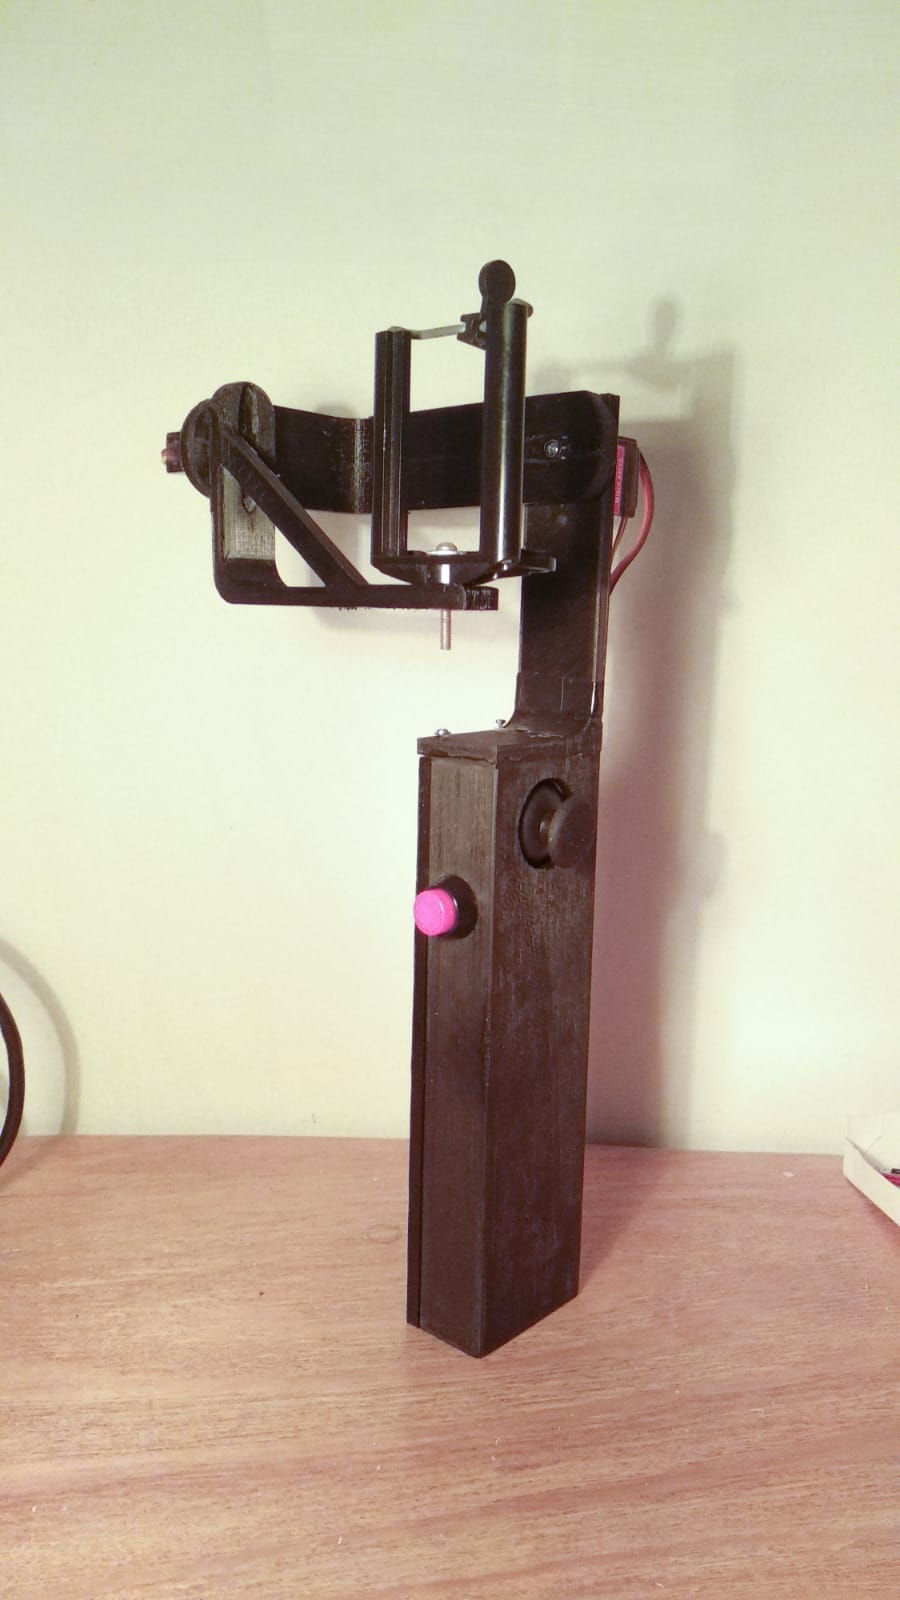
\includegraphics[width=0.4\textwidth]{Capitulo4 - Resultados/dir.jpeg}\\
\caption{\label{fig:widgets}Design final do dispositivo.}
\end{figure}

\begin{figure}[H]
\centering
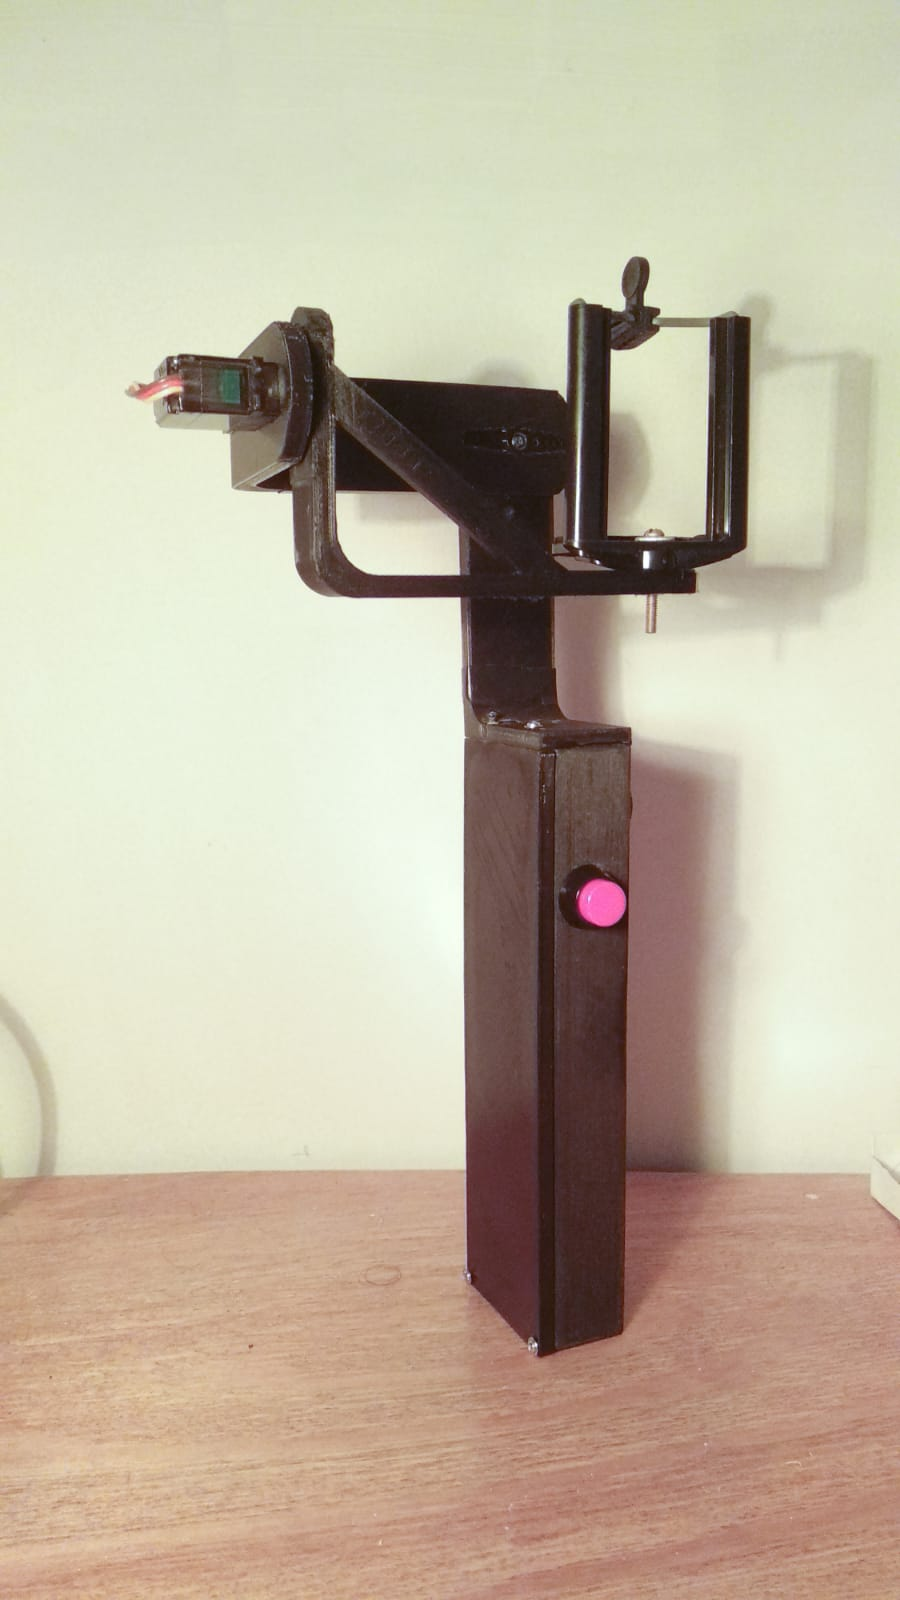
\includegraphics[width=0.4\textwidth]{Capitulo4 - Resultados/esq.jpeg}\\
\caption{\label{fig:widgets}Design final do dispositivo.}
\end{figure}